\section{Development and holdout results}\label{sec:results}

\subsection{Signal evidence and mechanism}

Table~\ref{tab:signals} and Figure~\ref{fig:mechanism} give the development evidence. All four signals have a positive IC at every horizon. The composite has an IC21 of 0.109 (hit rate 62\%, calibrated $p = 0.045$). LMH has the highest IC21 of the components, is positive in each of the three years, and is the only signal with a Fama-MacBeth $t$-statistic above two after the four price controls. The breadth signals lose significance once momentum is in the regression breadth on its own is largely momentum. The mechanism is directly visible: leader breadth predicts returns, herder breadth predicts reversals, and the difference collects both effects. Information builds over several weeks, with the composite's IC going from 0.026 at one session to 0.109 at 21.

\begin{table}[t]
\centering\small
\caption{Signal evidence development sample (2017-2019)}\label{tab:signals}
\begin{adjustbox}{max width=\textwidth}\begin{tabular}{lrrrrrrrrrr}
\toprule
 & IC5 & IC21 & IC63 & Hit (\%) & $t_{NW}$ & $t_{\text{phase}}$ & $p$ & Holm & Years $>0$ & FM $t$\\
\midrule
breadth\_63 & 0.036 & 0.072 & 0.064 & 61 & 1.50 & 1.16 & 0.127 & 0.30 & 2/3 & 0.21\\
event\_breadth\_63 & 0.033 & 0.085 & 0.082 & 58 & 1.73 & 1.26 & 0.108 & 0.30 & 2/3 & 0.15\\
breadth\_resid\_mom & 0.045 & 0.083 & 0.109 & 56 & 2.03 & 1.45 & 0.078 & 0.30 & 2/3 & 0.36\\
leader\_minus\_herd & 0.049 & 0.095 & 0.104 & 60 & 1.81 & 1.47 & 0.075 & 0.30 & 3/3 & 2.46\\
Composite & 0.053 & 0.109 & 0.114 & 62 & 2.19 & 1.74 & 0.045 & -- & 2/3 & 0.60\\
\quad leaders only & 0.039 & 0.066 & 0.051 & 57 & 1.28 & 1.03 & 0.155 & -- & 2/3 & 0.85\\
\quad herders only & $-0.123$ & $-0.084$ & $-0.148$ & 39 & $-0.78$ & -- & -- & -- & 0/3 & $-0.10$\\
\bottomrule
\end{tabular}\end{adjustbox}
\par\smallskip\begin{minipage}{0.97\textwidth}\footnotesize Mean daily Spearman rank IC with purged forward log returns. $t_{NW}$: Newey-West with 21 lags (shown for continuity it over-rejects). $t_{\text{phase}}$, $p$: calibrated phase-averaged non-overlapping test, one-sided. Holm: adjusted over the four components. FM $t$: Fama--MacBeth $t$ with controls for 12-1 and 6-1 momentum, 1-month reversal and 60-day volatility.\end{minipage}
\end{table}

\begin{figure}[t]
\centering
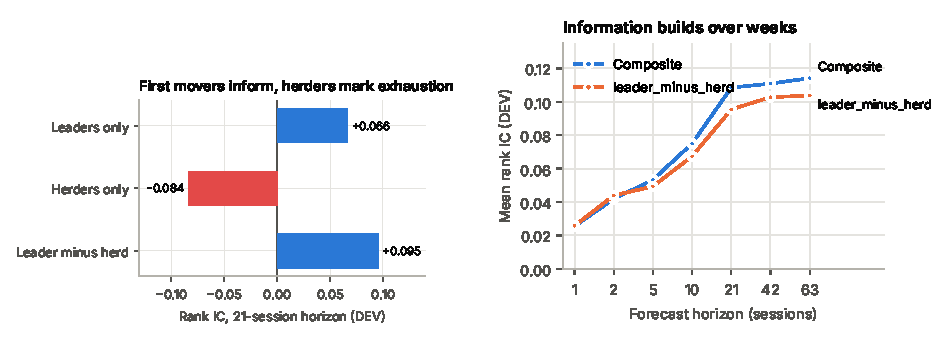
\includegraphics[width=\figw]{fig/fig02.pdf}
\caption{Mechanism and information horizon. Left: rank IC (21 sessions) of breadth from leader revisions only, herder revisions only, and their difference. Right: mean development IC of the composite and of LMH by horizon.}\label{fig:mechanism}
\end{figure}

\subsection{Construction and the price of the search}\label{sec:construction}

Table~\ref{tab:grid} and Figure~\ref{fig:grid} summarise the grid ($k\in\{3,4,5\}$, $f\in\{21,42,63,84,126\}$, equal or inverse-volatility weights). The rule fixed in advance picks $k=4$, $f=42$ and inverse-volatility weights, with a bootstrap-median Calmar of 0.855 against 0.735 for the equal-weight 63-session book. According to the diagnostics this choice is mostly cosmetic. It is also fragile in a literal sense. The rule keeps the lowest-turnover book within 0.02 of the best bootstrap median, and $k=4$ leads $k=5$ by little more than that. On a second machine, where re-estimated GARCH forecasts move the two medians to 0.840 and 0.825, the same rule picks $k=5$, whose 2017--2021 Sharpe ratio is 1.03 instead of 1.13. The book kept here ($k=4$) is the one frozen and pre-registered for the out-of-sample test, and the notebook now holds it fixed and reports when the rule would choose otherwise. The 30 books are near-duplicates (average correlation 0.91) and their in-sample ranking does not persist (PBO 0.945). The level does persist: the in-sample winner's median out-of-sample Sharpe ratio is 0.66. The deflated Sharpe ratio is 0.94 against the grid, 0.38 against the research log of 71 configurations, and 0.18 against all selection (Table~\ref{tab:dsr}). The development Sharpe ratio alone is not enough evidence, and this is why Sections~\ref{sec:toolkit} and~\ref{sec:oos} matter.

\begin{table}[t]
\centering\small
\caption{Development construction grid (top eight books)}\label{tab:grid}
\begin{adjustbox}{max width=\textwidth}\begin{tabular}{rrlrrrrrrr}
\toprule
$k$ & $f$ & Weights & Sharpe & CAGR (\%) & MaxDD (\%) & Calmar & Boot. median & Boot. 5\% & Turnover\\
\midrule
4 & 42 & IV-GJR $\blacklozenge$ & 0.98 & 7.7 & $-9.7$ & 0.79 & 0.85 & $-0.02$ & 2.1\\
5 & 42 & IV-GJR & 0.96 & 6.3 & $-7.7$ & 0.81 & 0.83 & 0.00 & 1.9\\
5 & 63 & IV-GJR & 0.96 & 6.1 & $-7.5$ & 0.81 & 0.81 & 0.00 & 1.4\\
4 & 63 & IV-GJR & 0.95 & 7.3 & $-9.6$ & 0.76 & 0.77 & $-0.05$ & 1.7\\
4 & 42 & EW & 0.91 & 8.1 & $-12.3$ & 0.66 & 0.77 & $-0.08$ & 1.7\\
5 & 63 & EW & 0.93 & 6.7 & $-8.7$ & 0.77 & 0.74 & $-0.06$ & 1.2\\
5 & 42 & EW & 0.88 & 6.4 & $-8.8$ & 0.73 & 0.74 & $-0.07$ & 1.5\\
4 & 21 & IV-GJR & 0.91 & 7.3 & $-10.5$ & 0.69 & 0.74 & $-0.07$ & 3.3\\
4 & 63 & EW (Round 3) & 0.92 & 8.0 & $-11.5$ & 0.69 & 0.73 & $-0.09$ & 1.4\\
\bottomrule
\end{tabular}\end{adjustbox}
\par\smallskip\begin{minipage}{0.97\textwidth}\footnotesize Dollar-neutral, net of 5\,bp. Boot.: Calmar across 1,000 stationary-bootstrap resamples of DEV. Turnover: one-way, times per year. $\blacklozenge$: selected.\end{minipage}
\end{table}

\begin{figure}[t]
\centering
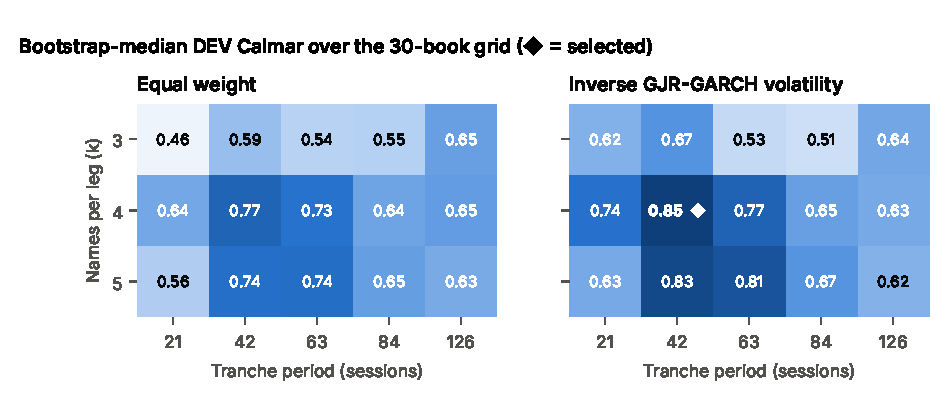
\includegraphics[width=\figw]{fig/fig03.pdf}
\caption{Bootstrap-median development Calmar ratio across the 30-book construction grid.}\label{fig:grid}
\end{figure}

\begin{table}[t]
\centering\small
\caption{Deflated Sharpe ratio of the selected book (development)}\label{tab:dsr}
\begin{adjustbox}{max width=\textwidth}\begin{tabular}{lrrrrr}
\toprule
Trial set & $N_{\text{eff}}$ & $SR_0$ (ann.) & Sharpe (ann.) & PSR(0) & DSR\\
\midrule
Within the 30-book grid & 3.5 & 0.07 & 0.98 & 0.95 & 0.94\\
Audit research log (71 configurations) & 37.2 & 1.15 & 0.98 & 0.95 & 0.38\\
All selection incl.\ pre-log ($\approx$284) & 250.2 & 1.51 & 0.98 & 0.95 & 0.18\\
\bottomrule
\end{tabular}\end{adjustbox}
\par\smallskip\begin{minipage}{0.9\textwidth}\footnotesize $SR_0$: expected maximum annualised Sharpe ratio of $N_{\text{eff}}$ independent null trials. Rows 2--3 use the cross-trial Sharpe dispersion of the research log.\end{minipage}
\end{table}

\subsection{Performance}

Table~\ref{tab:perf} and Figures~\ref{fig:equity}--\ref{fig:drawdown} compare the frozen book with its predecessors and with momentum. After costs FMF-N has Sharpe ratios of 0.98, 1.33 and 1.13 in DEV, the holdout and the full period, with volatility of 9.6\%, a maximum drawdown of $-14.1\%$, a beta of $-0.02$ and a Jensen alpha of 11.9\% a year ($t = 2.32$).
\begin{itemize}
  \item Compared with RTB's selection leg (Calmar 0.36, 0.85 and 0.53, gross of costs), FMF-N about doubles the development Calmar ratio and improves it in every window
  \item Compared with 12-1 momentum built the same way (full-period Sharpe 0.50, Calmar 0.23), FMF-N is more than twice as efficient
  \item Costs matter little: turnover is 2.1--2.7 times a year (10.8 for RTB), and the full-period Sharpe ratio is 1.16 gross and 1.11 at 10\,bp
\end{itemize}

\begin{table}[p]
\centering\small
\caption{Performance of the frozen specification and its predecessors}\label{tab:perf}
\begin{adjustbox}{max width=\textwidth}\begin{tabular}{lrrrrrrrrr}
\toprule
 & CAGR & Vol & Sharpe & MaxDD & Calmar & Beta & $\alpha$ (\%) & $t(\alpha)$ & PSR(0)\\
\midrule
\multicolumn{10}{l}{\emph{Panel A: DEV, 2017--2019}}\\
Revised strategy ($\tau=0$, net 5\,bp) & 7.7 & 7.9 & 0.98 & $-9.7$ & 0.79 & $-0.01$ & 8.2 & 1.82 & 0.95\\
\quad gross of costs & 7.9 & 7.9 & 1.01 & $-9.6$ & 0.82 & $-0.01$ & 8.4 & 1.87 & 0.96\\
\quad net 10\,bp & 7.5 & 7.9 & 0.95 & $-9.7$ & 0.77 & $-0.01$ & 8.0 & 1.77 & 0.95\\
Original selection component (gross) & 5.0 & 8.4 & 0.63 & $-13.9$ & 0.36 & $-0.07$ & 7.5 & 1.78 & 0.86\\
12-1 momentum, same construction (net) & 4.8 & 8.0 & 0.63 & $-11.5$ & 0.42 & 0.07 & 2.9 & 0.51 & 0.86\\
Original full strategy, HMM tilt (gross) & 16.6 & 10.2 & 1.56 & $-9.4$ & 1.77 & 0.20 & 10.2 & 2.46 & 1.00\\
Equal-weight market & 32.7 & 18.9 & 1.59 & $-25.1$ & 1.31 & 1.00 & -- & -- & 1.00\\
\midrule
\multicolumn{10}{l}{\emph{Panel B: Holdout, 2020--2021}}\\
Revised strategy ($\tau=0$, net 5\,bp) & 16.0 & 11.7 & 1.33 & $-14.1$ & 1.14 & $-0.14$ & 21.1 & 2.19 & 0.97\\
\quad gross of costs & 16.3 & 11.7 & 1.35 & $-14.0$ & 1.17 & $-0.14$ & 21.4 & 2.22 & 0.97\\
\quad net 10\,bp & 15.7 & 11.7 & 1.31 & $-14.1$ & 1.11 & $-0.14$ & 20.8 & 2.16 & 0.97\\
Original selection component (gross) & 13.2 & 13.3 & 1.00 & $-15.5$ & 0.85 & $-0.11$ & 17.5 & 2.07 & 0.92\\
12-1 momentum, same construction (net) & 5.2 & 14.2 & 0.43 & $-21.8$ & 0.24 & $-0.17$ & 12.4 & 1.15 & 0.72\\
Original full strategy, HMM tilt (gross) & 22.5 & 14.7 & 1.45 & $-13.6$ & 1.65 & 0.03 & 20.9 & 1.99 & 0.98\\
Equal-weight market & 34.1 & 32.1 & 1.08 & $-38.1$ & 0.89 & 1.00 & -- & -- & 0.93\\
\midrule
\multicolumn{10}{l}{\emph{Panel C: Full period, 2017--2021}}\\
Revised strategy ($\tau=0$, net 5\,bp) & 11.0 & 9.6 & 1.13 & $-14.1$ & 0.78 & $-0.02$ & 11.9 & 2.32 & 0.99\\
\quad gross of costs & 11.2 & 9.6 & 1.16 & $-14.0$ & 0.80 & $-0.02$ & 12.2 & 2.36 & 0.99\\
\quad net 10\,bp & 10.7 & 9.6 & 1.11 & $-14.1$ & 0.76 & $-0.02$ & 11.7 & 2.27 & 0.99\\
Original selection component (gross) & 8.3 & 10.6 & 0.80 & $-15.5$ & 0.53 & $-0.07$ & 10.9 & 2.35 & 0.96\\
12-1 momentum, same construction (net) & 5.0 & 10.9 & 0.50 & $-21.8$ & 0.23 & $-0.02$ & 6.4 & 1.00 & 0.86\\
Original full strategy, HMM tilt (gross) & 19.0 & 12.2 & 1.48 & $-13.6$ & 1.39 & 0.11 & 15.0 & 2.48 & 1.00\\
Equal-weight market & 33.3 & 25.0 & 1.28 & $-38.1$ & 0.87 & 1.00 & -- & -- & 1.00\\
\bottomrule
\end{tabular}\end{adjustbox}
\par\smallskip\begin{minipage}{0.97\textwidth}\footnotesize Percent per year for CAGR, volatility, drawdown and alpha. Beta and Jensen alpha from weekly regressions on the equal-weight market with HAC(4) errors. RTB figures are gross of costs.\end{minipage}
\end{table}

\begin{figure}[t]
\centering
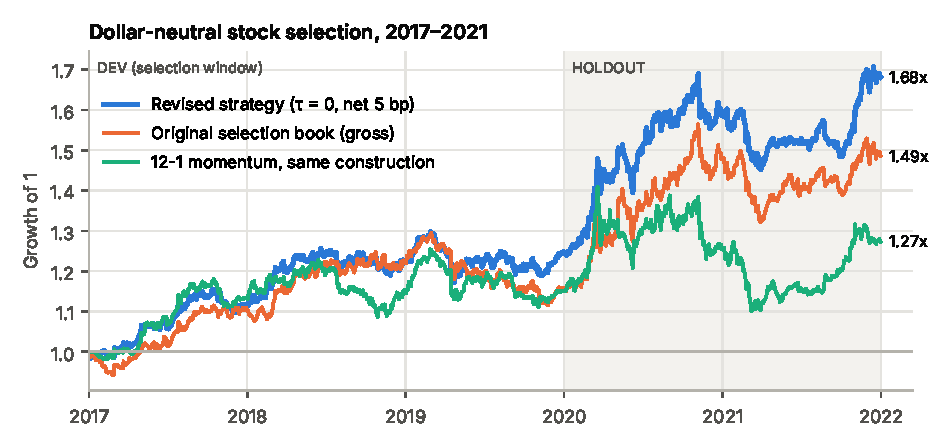
\includegraphics[width=\figw]{fig/fig04.pdf}
\caption{Growth of one unit, 2017--2021. FMF-N and 12-1 momentum are net of 5\,bp per unit traded; RTB's selection leg is gross. Shaded: holdout.}\label{fig:equity}
\end{figure}

\begin{figure}[t]
\centering
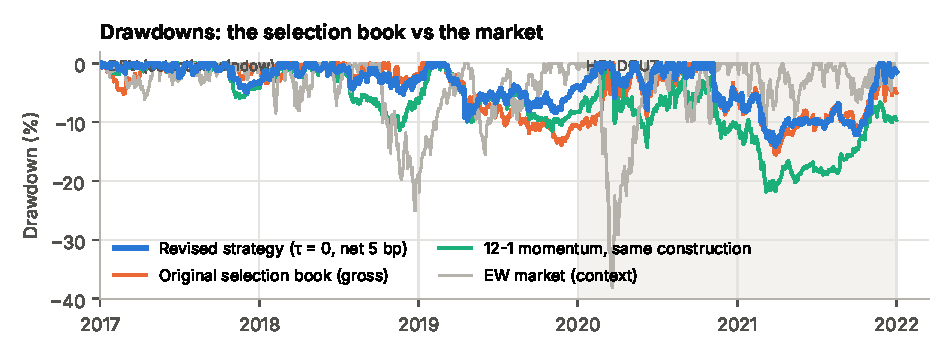
\includegraphics[width=\figw]{fig/fig05.pdf}
\caption{Drawdowns, 2017-2021, with the equal-weight market for context. In February-April 2020 the market's peak-to-trough return was $-38.1\%$, against $-5.8\%$ for FMF-N.}\label{fig:drawdown}
\end{figure}

\subsection{Attribution, placebos and concentration}

Against the market and four factor books built the same way from the price controls, FMF-N loads on 12-1 momentum (0.41) and against reversal ($-0.34$). These explain 0.60 of its variance, and an alpha of 7.4\% a year remains ($t = 2.98$; Table~\ref{tab:attrib}).
\begin{itemize}
  \item \emph{Placebos} (Table~\ref{tab:placebo}, Figure~\ref{fig:placebo}): FMF-N beats IID random scores and stock-label permutations in every window (full period $p = 0.003$ and $0.002$). Against the circular time-shift it passes in the holdout ($p = 0.025$) but not in DEV or over the full period ($p = 0.076$). Some of the edge is therefore which stocks the signal favours
  \item \emph{Leave-one-stock-out} (Table~\ref{tab:loo}, Figure~\ref{fig:loo}): Every rebuild runs the whole pipeline again on nine stocks. The full-period Sharpe ratio is between 0.80 and 1.25 (median 1.06). Without the largest P\&L contributor (stock\_6, about half of P\&L) the Sharpe ratio is 1.08 and the Calmar ratio 0.77. No single name carries the result
\end{itemize}

\begin{table}[t]
\centering\small
\caption{Factor attribution of the weekly book return}\label{tab:attrib}
\begin{adjustbox}{max width=\textwidth}\begin{tabular}{lrrrrrrrr}
\toprule
Window & $\alpha$ (\%) & $t(\alpha)$ & Market & Mom 12-1 & Mom 6-1 & Rev 1m & Low vol & $R^2$\\
\midrule
DEV & 6.0 & 2.33 & $-0.03$ & 0.67 & 0.08 & $-0.34$ & 0.08 & 0.67\\
Holdout & 12.3 & 2.03 & $-0.05$ & 0.20 & 0.26 & $-0.53$ & $-0.07$ & 0.63\\
Full & 7.4 & 2.98 & 0.02 & 0.41 & 0.25 & $-0.34$ & 0.05 & 0.60\\
\bottomrule
\end{tabular}\end{adjustbox}
\par\smallskip\begin{minipage}{0.9\textwidth}\footnotesize OLS on non-overlapping weekly returns, HAC(4) errors, factor books built with the strategy's construction.\end{minipage}
\end{table}

\begin{table}[t]
\centering\small
\caption{Placebo tests through the identical construction}\label{tab:placebo}
\begin{adjustbox}{max width=\textwidth}\begin{tabular}{llrrrrrrr}
\toprule
Window & Null & Draws & Sharpe & Null 95th & $p$ & Calmar & Null 95th & $p$\\
\midrule
DEV & IID random scores & 300 & 0.98 & 0.72 & 0.033 & 0.79 & 0.59 & 0.033\\
 & Stock-label permutation & 500 & 0.98 & 0.75 & 0.022 & 0.79 & 0.60 & 0.026\\
 & Circular time-shift & 315 & 0.98 & 1.39 & 0.146 & 0.79 & 1.52 & 0.146\\
Holdout & IID random scores & 300 & 1.33 & 0.80 & 0.010 & 1.14 & 0.69 & 0.017\\
 & Stock-label permutation & 500 & 1.33 & 0.98 & 0.016 & 1.14 & 1.06 & 0.044\\
 & Circular time-shift & 315 & 1.33 & 1.24 & 0.025 & 1.14 & 1.19 & 0.060\\
Full & IID random scores & 300 & 1.13 & 0.44 & 0.003 & 0.78 & 0.22 & 0.003\\
 & Stock-label permutation & 500 & 1.13 & 0.56 & 0.002 & 0.78 & 0.37 & 0.004\\
 & Circular time-shift & 315 & 1.13 & 1.21 & 0.076 & 0.78 & 1.05 & 0.076\\
\bottomrule
\end{tabular}\end{adjustbox}
\par\smallskip\footnotesize $p = (1+\#\{\text{null}\ge\text{observed}\})/(1+\text{draws})$.
\end{table}

\begin{figure}[t]
\centering
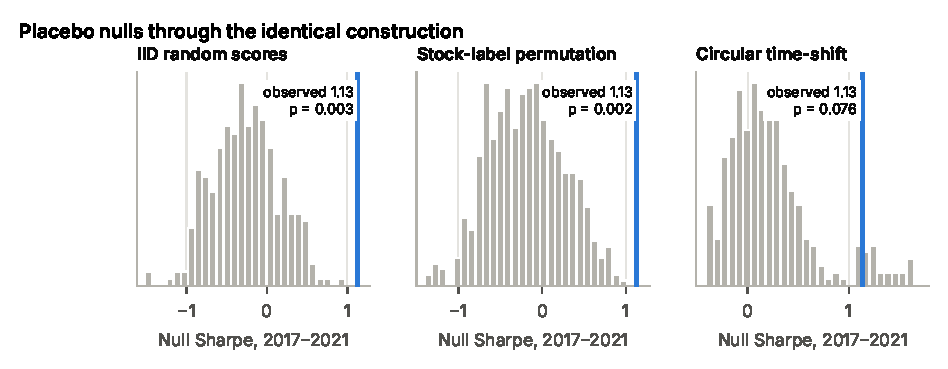
\includegraphics[width=\figw]{fig/fig06.pdf}
\caption{Full-period Sharpe ratios under the three placebo nulls; the line marks the observed value.}\label{fig:placebo}
\end{figure}

\begin{table}[t]
\centering\small
\caption{Full leave-one-stock-out rebuilds}\label{tab:loo}
\begin{adjustbox}{max width=\textwidth}\begin{tabular}{lrrrrrrrrr}
\toprule
 & \multicolumn{3}{c}{Sharpe} & \multicolumn{3}{c}{Calmar} & MaxDD & $\alpha$ & $t(\alpha)$\\
\cmidrule(lr){2-4}\cmidrule(lr){5-7}
Universe & DEV & Hold. & Full & DEV & Hold. & Full & Full (\%) & Full (\%) & Full\\
\midrule
All ten stocks & 0.98 & 1.33 & 1.13 & 0.79 & 1.14 & 0.78 & $-14.1$ & 11.9 & 2.32\\
without stock\_1 & 1.14 & 1.14 & 1.12 & 1.00 & 0.92 & 0.75 & $-14.7$ & 12.4 & 2.39\\
without stock\_2 & 0.58 & 1.10 & 0.81 & 0.47 & 0.96 & 0.62 & $-10.7$ & 5.5 & 1.37\\
without stock\_3 & 0.78 & 0.91 & 0.83 & 0.63 & 0.65 & 0.49 & $-14.3$ & 9.0 & 2.03\\
without stock\_4 & 0.90 & 0.72 & 0.80 & 0.77 & 0.50 & 0.46 & $-15.8$ & 8.6 & 1.72\\
without stock\_5 & 1.03 & 1.53 & 1.25 & 0.78 & 1.56 & 1.05 & $-11.4$ & 13.3 & 2.73\\
without stock\_6 & 0.87 & 1.34 & 1.08 & 0.66 & 1.18 & 0.77 & $-13.8$ & 10.6 & 1.98\\
without stock\_7 & 1.03 & 1.32 & 1.15 & 0.80 & 1.17 & 0.80 & $-14.1$ & 12.9 & 2.42\\
without stock\_8 & 0.80 & 1.27 & 1.02 & 0.63 & 1.16 & 0.73 & $-12.8$ & 10.4 & 1.99\\
without stock\_9 & 0.86 & 1.47 & 1.14 & 0.66 & 1.39 & 0.84 & $-12.5$ & 11.1 & 2.33\\
without stock\_10 & 0.98 & 1.15 & 1.04 & 1.23 & 0.91 & 0.65 & $-14.7$ & 10.3 & 2.13\\
\bottomrule
\end{tabular}\end{adjustbox}
\par\smallskip\begin{minipage}{0.95\textwidth}\footnotesize Each row repeats cleaning, calendar, snapshot, features, cross-sectional ranks, composite and allocation without one stock. GARCH forecasts are univariate and so do not change.\end{minipage}
\end{table}

\begin{figure}[t]
\centering
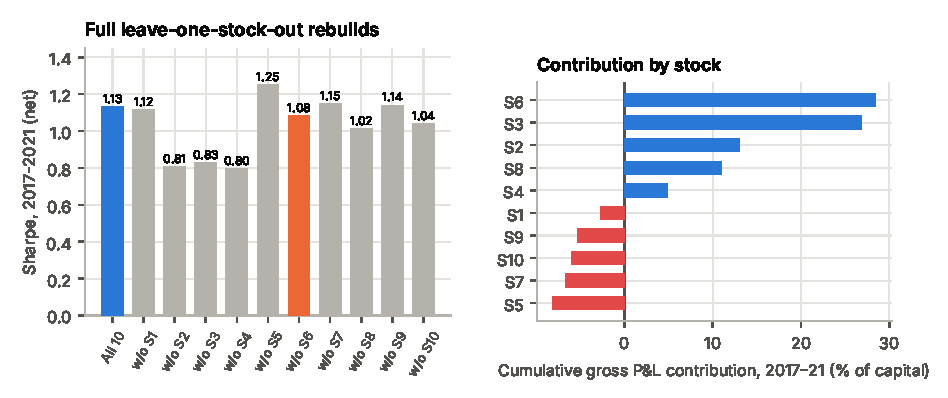
\includegraphics[width=\figw]{fig/fig07.pdf}
\caption{Left: full-period Sharpe ratio of the ten leave-one-stock-out rebuilds (orange: without the largest contributor). Right: cumulative gross P\&L by stock.}\label{fig:loo}
\end{figure}
